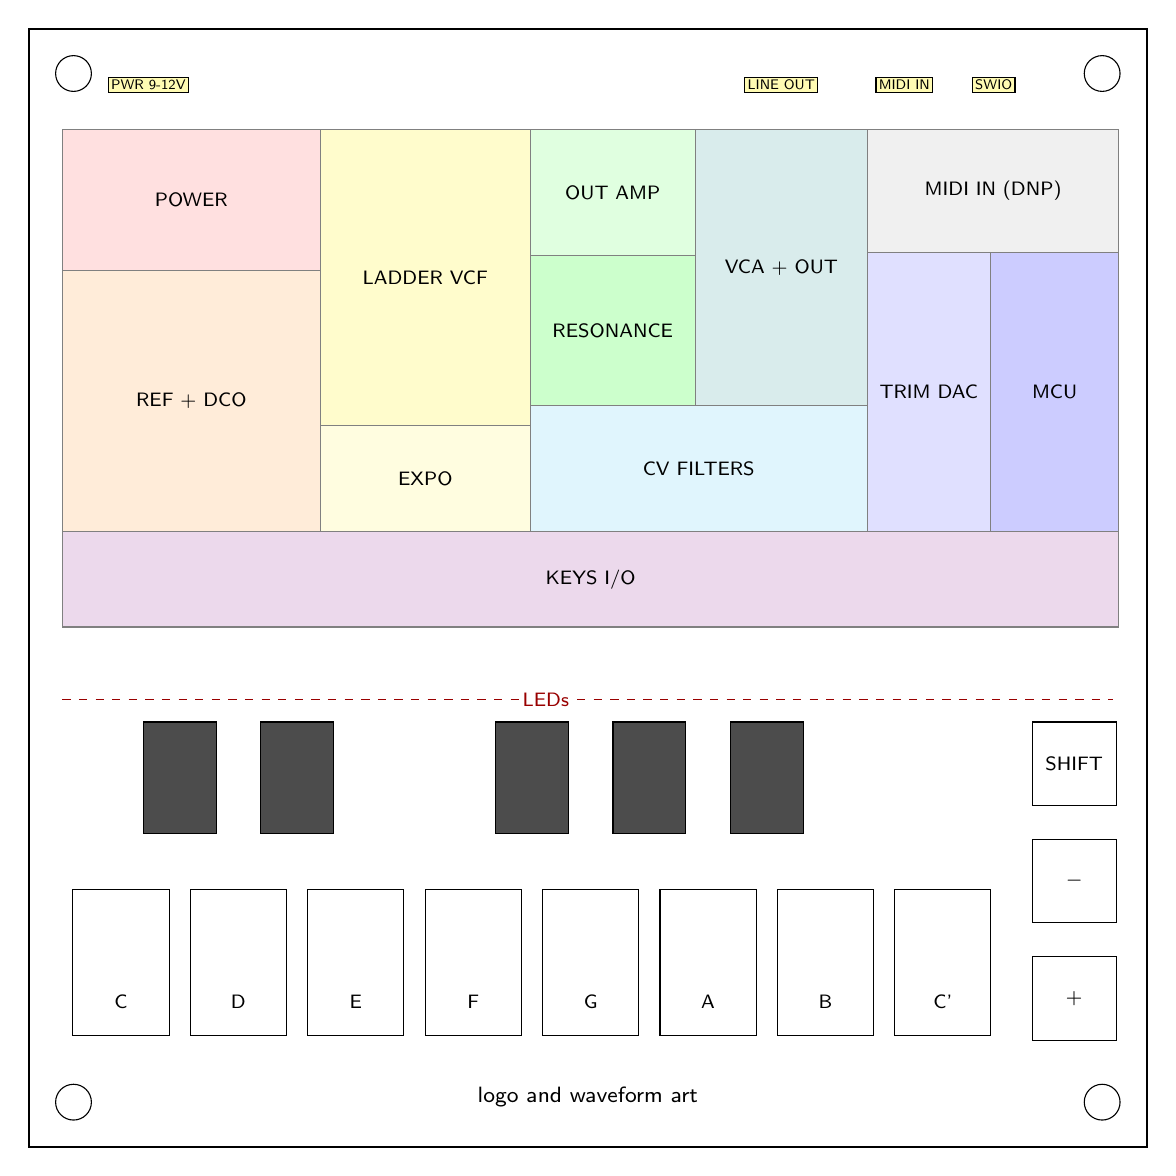
\begin{tikzpicture}[x=0.142cm,y=-0.142cm,font=\scriptsize\sffamily]
\draw[thick] (0,0) rectangle (100,100);
\filldraw[fill=red!12,draw=black!50] (3.00,9.00) rectangle (26.08,21.58);
\node[align=center,text width=2.95cm] at (14.54,15.29) {POWER};
\filldraw[fill=orange!15,draw=black!50] (3.00,21.58) rectangle (26.08,45.00);
\node[align=center,text width=2.95cm] at (14.54,33.29) {REF + DCO};
\filldraw[fill=yellow!20,draw=black!50] (26.08,9.00) rectangle (44.85,35.46);
\node[align=center,text width=2.40cm] at (35.46,22.23) {LADDER VCF};
\filldraw[fill=yellow!12,draw=black!50] (26.08,35.46) rectangle (44.85,45.00);
\node[align=center,text width=2.40cm] at (35.46,40.23) {EXPO};
\filldraw[fill=green!12,draw=black!50] (44.85,9.00) rectangle (59.62,20.28);
\node[align=center,text width=1.89cm] at (52.23,14.64) {OUT AMP};
\filldraw[fill=green!20,draw=black!50] (44.85,20.28) rectangle (59.62,33.72);
\node[align=center,text width=1.89cm] at (52.23,27.00) {RESONANCE};
\filldraw[fill=teal!15,draw=black!50] (59.62,9.00) rectangle (75.00,33.72);
\node[align=center,text width=1.97cm] at (67.31,21.36) {VCA + OUT};
\filldraw[fill=cyan!12,draw=black!50] (44.85,33.72) rectangle (75.00,45.00);
\node[align=center,text width=3.85cm] at (59.92,39.36) {CV FILTERS};
\filldraw[fill=gray!12,draw=black!50] (75.00,9.00) rectangle (97.50,20.00);
\node[align=center,text width=2.88cm] at (86.25,14.50) {MIDI IN (DNP)};
\filldraw[fill=blue!12,draw=black!50] (75.00,20.00) rectangle (86.00,45.00);
\node[align=center,text width=1.41cm] at (80.50,32.50) {TRIM DAC};
\filldraw[fill=blue!20,draw=black!50] (86.00,20.00) rectangle (97.50,45.00);
\node[align=center,text width=1.47cm] at (91.75,32.50) {MCU};
\filldraw[fill=violet!15,draw=black!50] (3.00,45.00) rectangle (97.50,53.50);
\node[align=center,text width=12.08cm] at (50.25,49.25) {KEYS I/O};
\draw[fill=white] (3.95,77) rectangle (12.55,90);
\node at (8.25,87) {C};
\draw[fill=white] (14.45,77) rectangle (23.05,90);
\node at (18.75,87) {D};
\draw[fill=white] (24.95,77) rectangle (33.55,90);
\node at (29.25,87) {E};
\draw[fill=white] (35.45,77) rectangle (44.05,90);
\node at (39.75,87) {F};
\draw[fill=white] (45.95,77) rectangle (54.55,90);
\node at (50.25,87) {G};
\draw[fill=white] (56.45,77) rectangle (65.05,90);
\node at (60.75,87) {A};
\draw[fill=white] (66.95,77) rectangle (75.55,90);
\node at (71.25,87) {B};
\draw[fill=white] (77.45,77) rectangle (86.05,90);
\node at (81.75,87) {C'};
\draw[fill=black!70] (10.25,62.00) rectangle (16.75,72.00);
\draw[fill=black!70] (20.75,62.00) rectangle (27.25,72.00);
\draw[fill=black!70] (41.75,62.00) rectangle (48.25,72.00);
\draw[fill=black!70] (52.25,62.00) rectangle (58.75,72.00);
\draw[fill=black!70] (62.75,62.00) rectangle (69.25,72.00);
\draw[fill=white] (89.75,62.00) rectangle (97.25,69.50);
\node at (93.50,65.75) {SHIFT};
\draw[fill=white] (89.75,72.47) rectangle (97.25,79.97);
\node at (93.50,76.22) {$-$};
\draw[fill=white] (89.75,82.95) rectangle (97.25,90.45);
\node at (93.50,86.70) {$+$};
\draw[dashed,red!60!black] (3,60.0) -- (97,60.0) node[pos=0.46,fill=white,inner sep=1pt] {LEDs};
\draw (4.0,4.0) circle (1.6);
\draw (96.0,4.0) circle (1.6);
\draw (4.0,96.0) circle (1.6);
\draw (96.0,96.0) circle (1.6);
\node[draw,fill=yellow!30,inner sep=1pt] at (10.7,5.0) {\tiny PWR 9-12V};
\node[draw,fill=yellow!30,inner sep=1pt] at (67.3,5.0) {\tiny LINE OUT};
\node[draw,fill=yellow!30,inner sep=1pt] at (78.3,5.0) {\tiny MIDI IN};
\node[draw,fill=yellow!30,inner sep=1pt] at (86.3,5.0) {\tiny SWIO};
\node[font=\footnotesize\sffamily] at (50,95.5) {logo and waveform art};
\end{tikzpicture}
